In our empirical investigation into the intricate relationship between gender, school composition, and post-secondary study decisions, we leverage comprehensive datasets from three primary sources: the Integrated School Enrollment System in Colombia (SIMAT), the National Higher Education Information System (SNIES), and the Formal Education Survey (EDUC).

The Integrated School Enrollment System in Colombia (SIMAT) serves as a fundamental resource in our research, providing detailed records of student enrollment and academic progress throughout their educational journey. This system offers a longitudinal perspective, enabling us to track individuals over time and analyze trends in educational outcomes.

Similarly, the National Higher Education Information System (SNIES) offers invaluable insights into post-secondary education in Colombia. With its extensive database of higher education institutions, programs, and student enrollment data, SNIES allows us to explore the majors students choose after completing secondary school. By examining enrollment patterns and graduation rates, we can better understand the dynamics of post-secondary education and its implications for future career paths.

To complement our analysis of individual-level data, we turn to the Formal Education Survey (EDUC), which provides detailed information about school attributes and educational environments. By examining factors such as school size, resources, and student demographics, we gain a more holistic understanding of the contextual nuances shaping the relationship between gender, school composition, and post-secondary study decisions.


In table \ref{tab:gender_dist2}, we present the distribution of students across different gender compositions in secondary schools. This table illustrates the proportion of male students in each school, ranging from 0 (representing single-gender female schools) to 1 (representing single-gender male schools). It is important to note that the values at the extremes (0 and 1) denote single-gender schools, which are excluded from the descriptive analysis. These single-gender schools lack sample variation within the school, thereby limiting their utility when calculating the relationship between studying a major and gender as a conditioning factor.

\begin{table}[!htbp] 
    \centering
    \begin{tabular}{cccccc}
    \hline \hline 
         Min. & 1st Qu. & Median  &  Mean & 3rd Qu.  &  Max.          \\\hline  \hline 
         0.000 &  0.377 & 0.462 & 0.457 & 0.546 &  1.000         \\
    \hline
    \end{tabular}
\caption{Proportion of Male Students in the Last Year of Secondary Schools}
\label{tab:gender_dist2}
\end{table}


 
 
From Figure \ref{histograma_male_fraction}, we observe a typical distribution representing the gender composition within classrooms, revealing an approximate mean with 46\% women. In it, we identify two main challenges. Firstly, single-gender schools transitioning to mixed schools encounter what we term 'corner decisions.' Secondly, students attending mixed schools, where classrooms have varying gender compositions, alter their post-secondary career choices due to gender reinforcement dynamics within the classroom.


\begin{figure}[H] % Use [h] to try to place the figure "here"
    \centering
    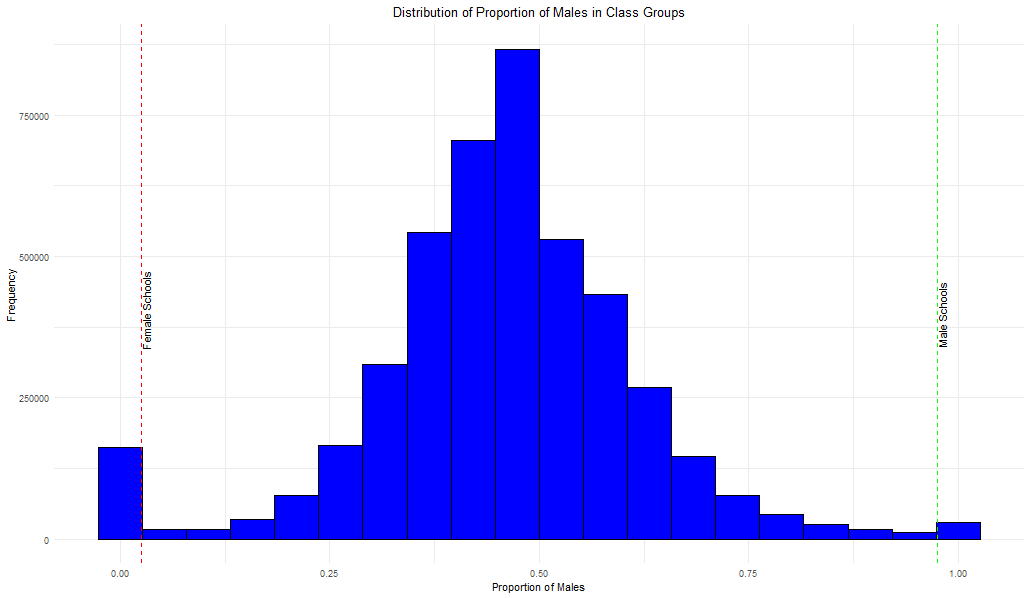
\includegraphics[width=0.7\linewidth]{Graph/his_frac_males.png} % Adjust width as needed
    \caption{Distribution of Proportion of Males in Class Groups}
    \label{histograma_male_fraction}
\end{figure}

